\documentclass[11pt]{article}

\usepackage{fullpage}
\usepackage{amsmath}
\usepackage{epsfig}
\usepackage{graphics}
\usepackage{caption}
\usepackage{circuitikz}

\oddsidemargin -0.15in
\evensidemargin -0.15in
\headheight 0in
\headsep 0in
%\topmargin -0.25in
\textheight 9.3in
\textwidth 6.8in

\begin{document}


\begin{center}
\section*{
Franklin \& Marshall College \hfill PHY 223\\
\bigskip
{\Large \it Interferometry 1}}
\end{center}
 
This experiment makes it possible for you to perform the famous two-slit
interference experiment with light, even in the limit of light intensities so
low that you can record the arrival of individual photons at the detector. You
perform three investigations:

\begin{enumerate}
\item You will be seeing two-slit interference visually, by opening up an
apparatus and seeing the exact arrangements of light sources and apertures that
operate to produce an ‘interference pattern’. You’ll be able examine every part
of the apparatus, and make all the measurements you’ll need for theoretical
modeling.

\item You will be able to perform the two-slit experiment quantitatively,
recreating not only Young’s measurement of the wavelength of light, but also
getting detailed information about intensities in a two-slit interference
pattern that can be compared to predictions of wave theories of light.

\item You will be able to perform the two-slit experiment one photon at a time,
continuing the same kind of experiments, but now at a light level so low that
you can assure yourself that there is at most one relevant photon in the
apparatus at any time. Not only will this familiarize you with single-photon
detection technology, it will also show you that however two-slit interference
is to be explained, it must be explained in terms that can apply to single
photons. (And how can a single photon involve itself with two slits?)
\end{enumerate}

You will explore goals 1 and 2 in the first week of this experiment, reserving
goal 3 for the second week.


\vspace{5mm}

\noindent {\bf Experimental setup}

The apparatus consists of a long rectangular metal assembly, with a single-photon
detection box attached at one end (see Fig. \ref{fig photo}).

\vspace{3mm}

\begin{minipage}{\linewidth}
  \centering
  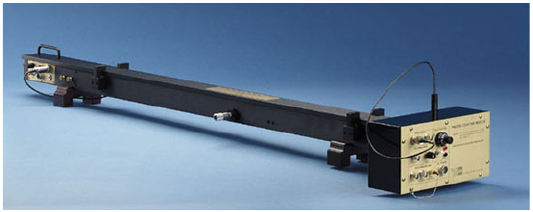
\includegraphics[scale=2.5]{Photo.png}
  \captionof{figure}{The TeachSpin two-slit interference device. The power
    supplies and light sources are to the left, the various slits are in the
    middle, and the photon detectors are on the right.}
  \label{fig photo}
\end{minipage}

\vspace{3mm}

First (before plugging anything in, or turning anything on) you’ll need to
confirm that the shutter that protects the amazingly sensitive single-photon
detector is closed. Locate the detector box at the right end of the apparatus,
and find the rod that projects out of the top of its interface with the long
assembly. Be sure that this rod is pushed all the way down; take this
opportunity to try pulling it vertically upward by about 2 cm, but then ensure
that it’s returned to its fully-down position. Also take this occasion to
confirm, on the detector box, that the toggle switch in the HIGH-VOLTAGE section
is turned off, and that the 10-turn dial near it is set to 0.00, fully
counter-clockwise.

Then open the cover and take a look inside. A schematic of the apparatus is
shown in Fig. \ref{fig schematic}. Make sure to identify the following parts:

\begin{itemize}

\item At the left end are two distinct light sources, one a red laser and the
other a green- filtered light bulb; also at the left end are the controls for
the light sources.
  
\item Along the length of the long box are the various slits and apertures that
form a Young’s two-slit experiment. On the front of the box are two ‘micrometer
drives’, which allow you to make mechanical adjustments to the two-slit
apparatus.

\item There are two distinct light detectors in the box at the right-hand end of
the apparatus:

  \begin{itemize}
  \item one is called the ‘photodiode’, which is used with the much brighter
laser light source; it’s attached to the light shutter in such a way that it’s
in position for use when the shutter is in its down position.

  \item the other is called the ‘photomultiplier tube’ or PMT for short, which
is used with the much dimmer light-bulb source. {\bf It is safe to use only when
the cover of the apparatus is in place and the light bulb is in use; it is
exposed to light only when the shutter is in the up position.}
  \end{itemize}

\item Finally, there are the electrical connections. Electric power comes from a
power module, plugged into your a.c. line and connected by a cable to the left
end of the apparatus. Two more cables run from this end to the detector box and
supply the photodiode and PMT detectors with the power they need for operation.
  
\end{itemize}

\vspace{3mm}

\begin{minipage}{\linewidth}
  \centering
  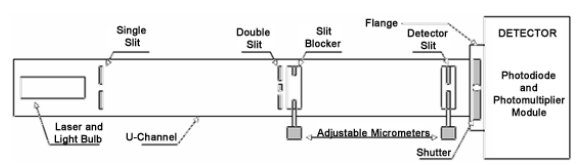
\includegraphics[scale=2.5]{Schematic.png}
  \captionof{figure}{Schematic diagram of the internal arrangement of the
    TeachSpin two-slit interference apparatus.}
    \label{fig schematic}
\end{minipage}

\vspace{5mm}

\noindent {\bf Procedure: Visual Mode}

For the visual mode of operation, you will be working with the cover of the
apparatus open. You will need to use neither light detector, since you will be
using your eyes as the only detector needed. You’ll be using the laser as light
source, and you’ll find a supply of small white paper screens to be convenient
tools.

Use the controls at the left end of the apparatus to turn on the solid-state
diode-laser light source—it’s contained within a black metal block. Use a paper
screen to find its bright red output beam; the diode laser manufacturer asserts
that its output wavelength is in the range from 650 nm to 675 nm, and its output
power is about 5 mW. (So long as you don’t allow the full beam to fall directly
into your eye, it presents no safety hazard.)

Follow the laser beam until it reaches the entrance slit, or ‘source slit’, of
the two-slit apparatus; this is a single slit of height about 1cm, but width of
only about a tenth of a mm. If you apparatus is aligned, the slit will be neatly
straddling the laser beam, so that a good fraction of the laser light will be
passing through the slit—use your paper screen to see if this is so.

Light passing through this narrow source slit will undergo ‘single-slit
diffraction’, and you can follow this process by moving your viewing card
downstream. You will see the red beam spread out horizontally, reaching a width
of about a cm by the time it reaches the middle of the apparatus.

In the middle of the apparatus is the holder for the double slit, which is a
structure with two rectangular apertures, again each about a cm high, and each
with width of about a tenth of a mm, and with center-to-center separation of
several tenths of a mm. [All of the slit structures are mounted on magnetic
holders so that they can be removed, examined, and re-positioned; if you
apparatus is already aligned (as yours is), it would be a pity to spoil this
alignment by disturbing the slits now.] Instead, put your viewing card just
downstream of the two-slit structure, and look (close up) to see if you can
observe the two ribbons of light, a few mm apart, which emerge from the two
slits.

This is your chance to understand the function of the slit blocker, just
downstream of the double-slit system, which will allow you selectively to block
the light coming from either of the two slits. This slit-blocker is controlled
by the ‘micrometer screw’ on the front center of the apparatus; rotating the
micrometer’s knob will move the slit-blocker laterally across the two ribbons of
light emerging from the two-slit system. For the present, find a position for
the micrometer adjustment that permits the two ribbons of light to emerge and
continue rightwards in the apparatus.

Each of the narrow ribbons of light emerging from a slit will continue to
diffract; follow these broadening ribbons downstream until they visibly overlap.
By the time your viewing card reaches the right-hand end of the apparatus, the
overlap will be nearly complete, and you’ll see that the two overlapping ribbons
of light combine to form a pattern of illumination displaying the celebrated
‘fringes’ named after Thomas Young.

Now position a viewing card at the downstream end so you can refer to it for a
view of the fringes, and take another card back upstream to the vicinity of the
slit-blocker. Learn to dial the slit-blocker’s micrometer adjuster [the one at
the middle of the apparatus] until you see how to use it to block the ribbon of
light coming from either the farther, or the nearer, of the two slits. Start by
rotating the multi-turn micrometer screw fully clockwise, and watch this
adjustment push the slit-blocker away from you.

{\bf Find and record the following five positions for the slit-blocker's
micrometer:}

\begin{itemize}
\item One position for which both slits are blocked.
\item Another for which light emerges from only the farthest of the two slits.
\item A third that allows light from both slits to propagate.
\item A fourth that only allows light from the nearest of the two slits.
\item A fifth that blocks from slits (on the other side).
\end{itemize}

\noindent You will need those position when you make measurements with the cover
back on.

At the far-right end of the apparatus is a final optical element; it’s an exit
slit, or ‘detector slit’, of the same size and character as the source slit,
except that it’s mounted on a moveable structure like the slit-blocker, so it
too can have its position adjusted by a micrometer screw drive. The purpose of
this detector slit is to allow light from a narrow slice of the interference
pattern to pass along to the end of the long apparatus and into the detector
box. By translating the detector slit laterally along the interference pattern
in space, you can select which part of the pattern will have its light sent on
to the detector. Thus by scanning the micrometer screw of the detector slit, you
can scan over the interference pattern, eventually mapping out its intensity
distribution quantitatively. For now, ensure that the detector slit is located
somewhere near the middle of the two-slit interference pattern.

\vspace{5mm}

\noindent {\bf Procedure: Quantitative Mode}

For this experiment, the box cover needs to be in place and the shutter of the
detector box will still be in its closed, or down, position. This blocks any
light from reaching the PMT, but the shutter in its down position correctly
centers a 1 cm solid-state photodiode, which acts just like a solar cell in
actively generating electric current when it’s illuminated. The device is
equally sensitive everywhere over its area, so it would record all the light in
the whole interference pattern if it were not for the detector slit. But with
the detector slit at a fixed position, the only light reaching the detector is
that from a selected part of the interference pattern; by this means, a single-
element, spatially-fixed, large-area detector can serve to record (serially in
time) the intensities at various places in the interference pattern. The method
of course relies on the fact that the rest of the apparatus is stable in time;
happily, the diode-laser source has an output power varying by $<$ 0.1\% in time,
and the mechanical stability of the rest of the apparatus is also adequate.

Connect a multimeter to the photodiode output on the detector box. You can test
whether or not the voltage you see is due to the light from the laser by
toggling the laser on and off. {\bf Record the value of the voltage when the
  laser is off.} You will need to subtract that from your measured values to
calculate the effect of the laser.

For the two-slit pattern, find the distance between interference maxima by
adjusting the position of the detector slit. Use that information to determine
the optimal step size for your actual measurement. Ideally, you want at least 10
data points between maxima. {\bf Then, scan the detector slit across the
  interference pattern, carefully noting the photodiode voltage at each
  location. Include 5 maxima in your scan.}

\vspace{5mm}

\noindent {\bf Modeling of interference and diffraction}

The simplest models for the data you have now taken are based on the assumptions
of Fraunhofer diffraction (see appendix below). The theory assumes light reaches
the double-slit assembly as a plane wave, ie. from a source infinitely far away.
In reality, your light reaches the double slits from the source slit, about 38
cm away.

The theory also assumes the double slits are the same width $a$, a center-
to-center separation labeled $d$, and are infinite. For your apparatus,
$a\approx 0.1$ mm, $d\approx 0.35$ mm, and the slit length is about 10 mm.
This is long enough that the effects of having a finite slit length can be
ignored.

The theory assumes the light is of a definite wavelength $\lambda$; in your
experiment, the laser light is monochromatic, with $\lambda$ between 650 nm and
670 nm. The filtered bulb light is not monochromatic, but is distributed over a
range from about 541 to 551 nm.

Theory assumes the light spreads from the double-slit assembly toward a point
detector also infinitely far away, so the radiation pattern can be expressed in
terms of an angular variable $\theta$, measured in radians from the central axis
of the apparatus. Your detector is not point-like, but is effectively 0.085 mm
wide; nor is it infinitely far away, but a distance of 49.95 cm downstream.
Nevertheless, it is approximately measuring light intensity as a function of an
angular variable; make a model that relates the theoretical parameter $\theta$
to the detector-slit position you can set with its micrometer.

The predicted intensity distribution derived from the assumptions of Fraunhofer
diffraction is

\begin{equation}
  I(\theta) = I_0\left( \cos\beta \right)^2\left( \frac{\sin\alpha}{\alpha}
  \right)^2
\end{equation}

\noindent where

\begin{equation}
  \alpha = \frac{\pi a}{\lambda}\sin\theta
\end{equation}

\begin{equation}
  \beta = \frac{\pi d}{\lambda}\sin\theta
\end{equation}

\noindent and $\theta$ is the angle of deflection of the light beam. 

Get some practice graphing this expression, until you understand the role of the
two factors in the intensity expression; also, get familiar enough with its
derivation that you can understand how the theoretical prediction changes when
one, or the other, of the two slits are blocked.

The theory doesn’t pretend to give the intensity $I_0$ at central maximum,
whether that’s in units of photodiode voltage or photon count rate; so you can
supply this value to the theory ``by hand''. The theory also can’t know what
setting of your detector-slit micrometer corresponds to the location of the
two-slit pattern’s central maximum, so you can provide this value ‘by hand’ as
well. But with these vertical-scale and horizontal- zero adjustments, you should
be able to inter-compare theoretical predictions and experimental data for
signals as a function of detector-slit position.

There are much more sophisticated theoretical models than this one. In
particular, there are discussions of Fresnel-diffraction and sum-over-paths
models that avoid some of the approximations made above. Nevertheless, these
more sophisticated models do not change any qualitative conclusions you have
established, and they make only the slightest quantitative differences to your
predictions; the need for deep thought about duality for light remains just as
urgent after the models for its behavior have been improved.

\vspace{5mm}

\noindent {\bf Analysis}

You can read the appendix (``Fraunhofer diffraction'') below to refresh your
knowledge of diffraction and interference before analyzing your results.

\begin{itemize}
\item Use the positions of the double-slit minima.
\item Plot the positions of the minima vs. its order ($m$). Use the slope of that
  graph to calculate the slit separation $d$ with uncertainty.
\item Plot your double-slit data to show the double-slit interference pattern.
\item Superpose your data plot with a model of your results (calculated from the
  equations in the appendix) with the central intensity, central location, slit
  spacing, and slit width parameters optimized to agree with your data. Estimate
  the uncertainty in the slit spacing parameter required. (You can use the
  following starting values: $a\approx0.1$ mm and $d\approx0.35$ mm.)
\item Compare your two results for slit spacing.
\end{itemize}

\noindent {\bf To submit}

\begin{enumerate}
\item A properly formatted graph (axes, labels, error bars, etc) 
showing of position of the minima as a function of order ($m$) which include 
the best fit line.

\item A calculation of of the slit width $d$ with uncertainty from the 
results of the previous graph.

\item A properly formatted graph (axes, labels, error bars, etc) 
showing of position of the interference pattern with at least 5 fringes and 
ten data points per fringe. Add a modeling line on top of the data according
to Eq. \ref{eq: I(y)}.

\item A brief discussion of the size of the uncertainty. Is it reasonable? 
Why/why not? What are likely the most common sources of error? What improvements 
could you do to the apparatus or to how it's used to reduce the size of the 
error. 
\end{enumerate}

\newpage

\noindent {\bf Appendix: Fraunhofer diffraction}

\vspace{3mm}

\begin{minipage}{\linewidth}
  \centering
  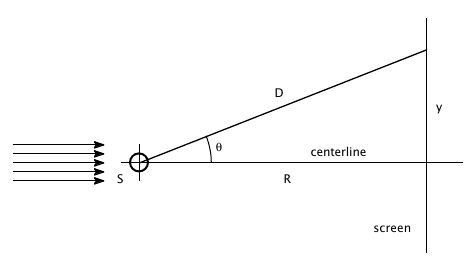
\includegraphics[scale=2.5]{Diffraction.png}
  \captionof{figure}{Geometry of Fraunhofer diffraction. An incoming parallel
    beam is incident on a slit structure S and diffracts to hit a screen at
    height $y$ above the centerline.}
  \label{fig diffraction}
\end{minipage}

\vspace{3mm}

In this appendix we will review how to analyze the single-slit and two-slit
interference patterns using the assumptions of Fraunhofer diffraction. The
geometric configuration is shown in Fig. \ref{fig diffraction}. The incoming
monochromatic light, of wavelength $\lambda$, is incident from the left. We
assume that the light arrives as a plane wave, which means in practice that the
source of the incident light is far to the left. The incoming light is incident
on a slit arrangement S, which is assumed to be infinitesimally small compared
to the other distances ($R$, $D$, $y$) of the scattering. The slit arrangement S
is a source for scattered waves, one of which is shown going at angle $\theta$ relative
to its original direction. A screen is shown to the right in the diagram at
distance $R$ from the scattering center S. The scattered wave travels a distance
$D$ before hitting the screen a distance $y$ above the centerline. We will
assume that the amplitude of the scattered wave is independent of $y$, which is
saying that $D$ doesn’t vary much from $R$, or that the angle $\theta$ is small.
The
trigonometric relations are

\begin{equation}
  \tan\theta = \frac{y}{R}
\end{equation}

\noindent and

\begin{equation}
  \sin\theta = \frac{y}{D}
\end{equation}

Slit arrangements have some structure so that the wave arriving on the screen at
$y$ is a sum of contributions coming from the various slit parts. In Fig.
\ref{fig interference} a particular wave, coming from an opening located a
distance $h$ above the centerline, is shown. This wave moves a distance $d$,
which is slightly different from $D$, in order to reach the screen a distance
$y$ above the centerline. (The vertical dimension is exaggerated in this diagram
for clarity.)

\vspace{3mm}

\begin{minipage}{\linewidth}
  \centering
  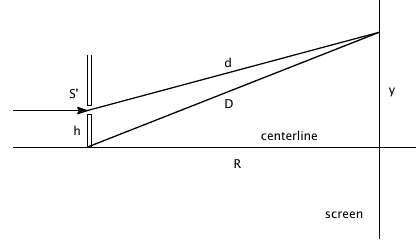
\includegraphics[scale=2.5]{Interference.png}
  \captionof{figure}{Details of the slit structure in Fraunhofer diffraction.
    Variations in the wave travel distance d will be important for determining
    the phase of the wave on the screen.}
  \label{fig interference}
\end{minipage}

\vspace{3mm}

Waves scattered at the slit structure spread out with a spherical wavefront and
are described by the spherical wave $\Psi = \chi e^{i(kd-\omega t)}$, where $k =
2\pi/\lambda$ is the wave number, $\omega = 2\pi f$ is the angular frequency,
and $\chi$ is the differential amplitude coming from this small contribution to
the total scattered wave. We use a complex exponential form to describe the
wave, but we could have used a real form by working with the real part of
$\Psi$. The complete wave arriving at any point on the screen is a sum of
contributions coming from the various parts of the slit structure. This total
contribution is given by the sum

\begin{equation}
  \Psi(y) = A\int_{slit}dh e^{i(kd-\omega t)}
\end{equation}

\noindent where $(Adh)e^{i(kd-\omega t)}$ is the small wave contribution coming
from a differential length $dh$ of the slit. We have assumed that the quantity
$A$ is a constant (independent of $h$ and $y$, which means we are assuming that
the distances between the various parts of the slit structure to the a point on
the diffraction pattern on the screen are nearly the same. However, the effects
of variations in $d$ in the exponential are significant and we take them into
account. We can write

\begin{equation}
  d = \left( R^2+(y-d)^2 \right)^{1/2} = \left( R^2+y^2-2yh+h^2
  \right)^{1/2} \approx D\left( 1-\frac{yh}{D} \right)
\end{equation}

for small $\theta$ (that is, for $y/D << 1$ ) and small $h$ (that is, for
$h/D<<1$), so that

\begin{equation}
  \Psi(y) \approx Ae^{i(kD-\omega t)} \int_{slit}dh e^{-ikyh/D}
\end{equation}

We have defined $D = (R^2+y^2)^{1/2}$. As a first application of this
``Fraunhofer'' diffraction, we calculate the diffraction pattern formed from a
double slit arrangement. We take a slit width a and a slit separation $d$, so
the slit is open for $-(d+a)/2<h<-(d-a)/2$ and $(d-a)/2<h<(d+a)/2$. The wave at
height $y$ on the screen is

\begin{equation}
  \Psi(y) = Ae^{i(kD-\omega t)}\left( \int_{-(d+a)/2}^{-(d-a)/2}dh e^{-ikyhD} +
  \int_{(d-a/2)}^{(d+a)/2}dh e^{-ikyh/D} \right)
\end{equation}

This integral can be done with the result

\begin{equation}
  \Psi(y) = 2aA e^{kD-\omega t}\frac{\sin\alpha}{\alpha}\cos\beta
\end{equation}

\noindent where

\begin{equation}
  \alpha = \frac{\pi a}{\lambda}\sin\theta = \frac{kya}{2D}
\end{equation}

\begin{equation}
  \beta = \frac{\pi d}{\lambda}\sin\theta = \frac{kyd}{2D}
\end{equation}

\noindent and we have used the Euler identities

\begin{equation}
  e^{i\theta} + e^{-i\theta} = 2\cos\theta
\end{equation}

\noindent and

\begin{equation}
  e^{i\theta} - e^{-i\theta} = -2i\sin\theta
\end{equation}

\noindent The intensity is the complex square of the wave amplitude. For the
double slit we have

\begin{equation}
  I(y) = I_0\left( \frac{\sin\alpha}{\alpha} \right)^2\left( \cos\beta \right)^2
  \label{eq: I(y)}
\end{equation}

\noindent where $I_0 = 4|aA|^2$ is the maximum of the intensity distribution,
which occurs at $y=0$.

The distribution for a single slit, located at $-a/2<h<a/2$, is given by

\begin{equation}
  \Psi(y) = Ae^{i(kD - \omega t)}\int_{-a/2}^{a/2}dh e^{-ikyd/D} =
  aA e^{i(kD - \omega t)}\frac{\sin\alpha}{\alpha}
\end{equation}

with corresponding intensity distribution

\begin{equation}
  I(y) = \frac{I_0}{4}\left( \frac{\sin\alpha}{\alpha} \right)^2
\end{equation}
\end{document}
